\documentclass[a4paper,12pt]{article}
\usepackage[utf8]{inputenc}
\usepackage[brazil]{babel}
\usepackage[lmargin=3cm,tmargin=3cm,rmargin=2cm,bmargin=2cm]{geometry}
\usepackage[T1]{fontenc}
\usepackage{amsmath,amsthm,amsfonts,amssymb,dsfont,mathtools}
\usepackage{blindtext}
\usepackage{graphicx} % Required for inserting images

\begin{document}


\begin{center}
\textbf{FATEC RUBENS LARA}

\textbf{CURSO DE CIÊNCIA DE DADOS}

\vspace{3cm}

\section*{Principal Component Analysis (PCA)}
\subsection*{Análise de Padrões Estratégicos: Explorando o Potencial do PCA no Cenário Competitivo de Esportes Eletrônicos}



\vspace{3cm}

\textbf{GUSTAVO FERREIRA GONÇALVES LIMA}

\textbf{GUSTAVO MIRANDA SILVA}

\textbf{ISABELA VIEIRA DA SILVA CRUZ MARTINS}





\vfill

\begin{flushright}
Santos - São Paulo\\
27/11/2023
\end{flushright}
\end{center}
\begin{figure}{}
\centering
\label{}

\includegraphics[width=14cm,height=2cm]{rodap-4.png}
\end{figure}
\pagebreak

\section{Definição}
A análise de componentes principais (PCA) é uma ferramenta padrão na análise moderna de dados e é utilizada por quase todas as disciplinas científicas. O objetivo do PCA é identificar a base mais significativa para reexpressar um conjunto de dados apresentado. Espera-se que essa nova base revele estruturas ocultas no conjunto de dados e filtre o ruído. Existem muitas aplicações, como redução de dimensionalidade, compressão de dados, extração de características e visualização de dados.
\section{Extração dos componentes principais}
Para se extrair as componentes principais, são submetidos os seguintes passos:
\subsection{Padronização dos Dados:}

Assegura-se de que todas as variáveis tenham média zero e desvio padrão igual a um, colocando-as na mesma escala.
\subsection{Matriz de Covariância:}

Calcula-se a matriz de covariância ao utilizar os dados padronizados, de modo que revele as relações entre as variáveis.
\subsection{Autovalores e Autovetores:}

Encontram-se os autovalores e autovetores da matriz de covariância, de maneira que represente a variância explicada por cada componente principal e a direção dessas componentes.
\subsection{Ordenação dos Autovalores:}

Colocam-se os autovalores em ordem decrescente para destacar os mais significativos, que correspondem a mais variância nos dados.
\subsection{Seleção dos Componentes Principais:}

Decide-se quantos dos maiores autovalores (e seus autovetores correspondentes) serão mantidos, de modo que determine assim o número de componentes principais.
\subsection{Construção da Matriz de Projeção:}

Forma-se uma matriz com os autovetores escolhidos, em que cada coluna representa uma componente principal. Essa matriz de projeção define a transformação dos dados.
\subsection{Transformação dos Dados Originais:}

Projetam-se os dados originais no novo espaço definido pelas componentes principais, de forma a realizar a multiplicação da matriz de dados pela matriz de projeção.
\section{Uso do PCA}
Para realizar a aplicação de um PCA, foi escolhido um conjunto de dados sobre o campeonato mundial de League of Legends (LoL) de 2022. Este é um jogo do gênero Multiplayer Online Battle Arena (MOBA), lançado em 2009. A princípio, sua partida tem o formato de 5x5 constitúido de dois times, sendo eles um do lado azul, e o outro do lado vermelho, e cada lado possui características próprias que auxiliam na vitória.\\ Durante o campeonato, os times tem o direito de banir campeões de forma estratégica para mitigar as opções de escolhas e/ou respostas do time inimigo. Os jogadores escolhem entre os 157 campeões distintos disponíveis para a jogabilidade no ano comentado.\\No conjunto de dados citado foram selecionados os 22 campeões de LoL que mais foram presentes em requisitos de escolha e banimento. Suas colunas apresentam quantificações de banimentos, escolha, taxa de vitória e taxa de derrota, taxa de vitória no lado azul e vermelho, taxa de derrota no lado azul e vermelho, também como colunas que apresentam razões entre escolha e banimento, vitória e derrota.\\
Para a realização do estudo foi utilizado a ferramenta PAST, uma ferramenta estatística ampla. Ela oferece uma variedade de métodos estatísticos e ferramentas de visualização, que inclui análise de variância, regressão e análise de componentes principais. Além dela usufrui-se para normalização dos dados o Excel, e o python para obtenção dos valores da matriz de covariância e dos autovetores.

\subsection{Normalização dos Dados}
O escore padrão (também conhecido como escore Z ou escore Z-padronizado), é calculado de modo que se use a fórmula do escore Z. O escore Z mede o número de desvios padrão que um determinado valor está em relação à média de um conjunto de dados. A fórmula para calcular o escore Z é dada por:

\[ Z = \frac{{X - \mu}}{{\sigma}} \]

onde:
- \( Z \) é o escore Z,\\
- \( X \) é o valor individual,\\
- \( \mu \) é a média do conjunto de dados,\\
- \( \sigma \) é o desvio padrão do conjunto de dados.\\

Essa fórmula transforma os dados originais em uma escala em que a média é 0 e o desvio padrão é 1. Isso é útil para normalizar os dados e comparar valores de diferentes conjuntos que podem ter unidades ou escalas diferentes.\\
Ao aplicar a fórmula do escore Z a cada valor de uma variável, obtém-se uma distribuição que é centrada na média 0 e tem uma dispersão padronizada. Essa normalização é valiosa ao realizar análises estatísticas e técnicas como o PCA, onde a consistência nas escalas das variáveis é essencial para interpretações significativas.\\

\begin{figure}[h]
Na figura abaixo temos uma pequena demonstração em 5 colunas das 17 presentes no dataset, com os dados normalizados ao se aplicar o zscore em cada individualmente:\\\\
    \centering
    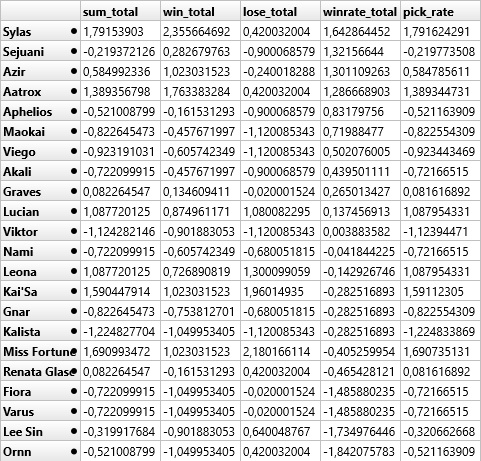
\includegraphics{Dataset.jpg}
    \caption{Ferramenta PAST}
    \label{fig:enter-label}
\end{figure}

A normalização dos dados desempenha um papel crucial na análise de componentes principais (PCA), especialmente ao lidar com conjuntos de dados que possuem variâncias e escalas diferentes entre suas variáveis. Ao normalizar os dados, garantimos que todas as variáveis contribuam de maneira equitativa para a análise, uma vez que passam a compartilhar a mesma escala. Isso é essencial no contexto do PCA, onde o objetivo é identificar as direções de maior variância nos dados.\\
Assim, a normalização não apenas equaliza o peso das variáveis, o que permite uma análise mais justa, mas também assegura que a matriz de covariância captura adequadamente as relações entre as variáveis, e se resulta em componentes principais mais representativos e informativos.\\

\subsection{Matriz de Covariância}
A normalização também desempenha um papel significativo ao utilizar a matriz de covariância na análise. A matriz de covariância é fundamental para calcular os autovetores e autovalores no PCA, o que influencia diretamente a identificação das direções principais nos dados. Se os dados não forem normalizados, variáveis com escalas mais altas podem dominar a contribuição para a matriz de covariância, o que leva a resultados distorcidos e pouco representativos.
\pagebreak
\begin{center}
Matriz de Covariância Reduzida:\\\\
\begin{bmatrix}
1 & 0.92207786 & 0.81812014 & 0.30969505 & 0.99999992 \\
0.92207786 & 1 & 0.53182461 & 0.64040849 & 0.92207323 \\
0.81812014 & 0.53182461 & 1 & -0.2738949 & 0.81812686 \\
0.30969505 & 0.64040849 & -0.2738949 & 1 & 0.30967666 \\
0.99999992 & 0.92207323 & 0.81812686 & 0.30967666 & 1 \\
\end{bmatrix}
\end{center}



\subsection{Autovetores}
Os autovetores desempenham um papel crucial ao definir as novas direções (componentes principais) ao longo das quais os dados têm a máxima variância. Cada autovetor corresponde a uma dessas direções, e seus componentes indicam a contribuição relativa de cada variável original nessa direção específica.\\
Os autovetores são derivados da matriz de covariância dos dados normalizados. A matriz de covariância captura as relações lineares entre as variáveis originais, e os autovetores fornecem as direções em que essas relações são mais expressivas.\\
Os autovetores são ordenados de acordo com os autovalores associados, que indicam a quantidade de variância explicada por cada componente principal. Os dois maiores autovetores, portanto, correspondem às direções de máxima variância nos dados.\\
Os dois maiores auto vetores:\\
\[
\begin{bmatrix}
0.31296824 & 0.29253293 & 0.25017361 & 0.10426059\\
0.31296515 & 0.28317626 & 0.26656886 & 0.21117737 \\
0.10769845 & 0.21911506 & 0.18662749 & 0.16034463 \\
0.01024246 & 0.2677644 & 0.26776522 & 0.30461193 & 0.30461107 
\end{bmatrix}
\]
\[
\begin{bmatrix}
-0.00309909 & -0.21691925 & 0.31553737 & -0.54420917\\
-0.00310578 & -0.13038932 & -0.19061426 & 0.02024007\\
-0.14635182 & 0.19520773 & -0.15111444 & 0.45295414\\
-0.0452074 & 0.06241295 & 0.06243902 & -0.04338876 & -0.04334922 
\end{bmatrix}
\]
\subsection{AutoValores}

Na Ferramenta PAST temos a opção de calcular o PCA de duas formas, através de uma matriz de covariância ou correlação, porém como explicado anteriormente será usada a matriz de covariância, pois os dados estão normalizados com escalas equilibradas.\\
Abaixo pode ser observado o cálculo de 17 componentes principais, com seus autovalores e a variância que cada um representa dos dados originais. Neste caso, será utilizado apenas os dois primeiros componentes principais, uma vez que os restantes dos componentes representam um número insignificante de informações do conjunto de dados. Isto é, se somados, os PC1 e PC2, representam aproximadamente 73\% da massa de dados.

\begin{figure}[h]
    \centering
    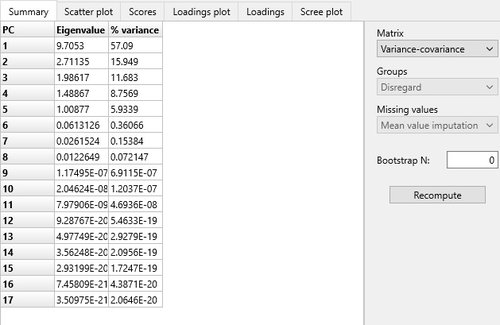
\includegraphics{Pc1Pc2 (1).jpg}
    \caption{Ferramenta PAST}
    \label{fig:enter-label}
\end{figure}


\pagebreak
\section{Resultados}
Para analisar as variáveis fornecidas dentro do PCA, há dois gráficos de coluna que quantificam os loadings em cada componente, os "loadings" em uma análise de Componentes Principais (PCA) indicam a contribuição de cada variável para a formação de um determinado componente principal. Em termos mais simples, eles representam a relação entre as variáveis originais e os componentes principais calculados durante o PCA.\\
Em um componente principal específico, os loadings mostram o peso relativo de cada variável na criação desse componente. Valores mais altos indicam uma contribuição mais significativa da variável para a variação capturada pelo componente principal. Portanto, para interpretar os loadings, identifica-se quais variáveis têm maior influência na direção específica de variação representada pelo componente principal.\\
Neste estudo específico, os loadings podem ser utilizados para compreender quais métricas ou características específicas dos campeões de um jogo (como taxa de escolha, taxa de vitórias, etc.) estão mais fortemente associadas a certos padrões ou comportamentos identificados pelos componentes principais.\\

\begin{figure}[h]
Na figura 3 abaixo temos o grafico de coluna referente aos loadings de PC1:
    \centering
    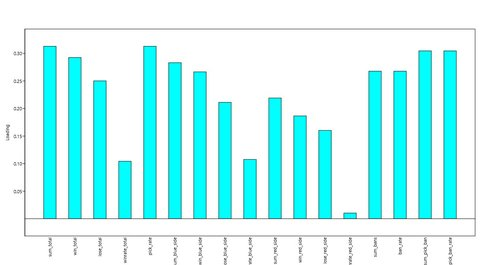
\includegraphics{LoadingsPC1 (1).jpg}
    \caption{Ferramenta PAST}
    \label{fig:enter-label}
\end{figure}
\pagebreak
Os quatro maiores valores em PC1, que representam a direção de maior variância nos dados, são:\\

1. \textbf{pick\_rate (0.31):} Indica a taxa de escolha de campeões, o que contribui significativamente para a variação geral nos dados.\\

2. \textbf{sum\_total (0.31):} Reflete a soma total de algumas métricas não especificadas, também desempenhando um papel crucial na variabilidade.\\

3. \textbf{sum\_pick\_ban (0.30):} A soma de escolhas e bans é a terceira variável mais influente em PC1.\\

4. \textbf{pick\_ban\_rate (0.30):} A taxa de escolha e ban também tem um valor significativo em PC1, de forma que contribua consideravelmente para a variação nesse componente.\\



\begin{figure}[h]
Ao relacionarmos PC1 com PC1 em um gráfico temos a seguinte figura abaixo:
    \centering
    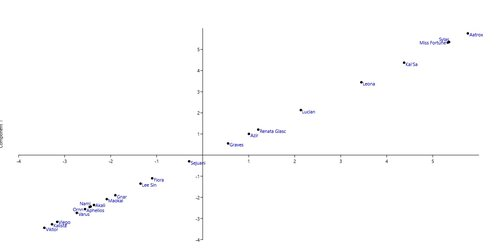
\includegraphics{Pc1Pc1 (1).jpg}
    \caption{Ferramenta PAST}
    \label{fig:enter-label}
\end{figure}
\pagebreak
\begin{figure}[h]
Para compreensão, serão selecionados 3 das amostras para analisar seus valores brutos como feito na figura abaixo:
    \centering
    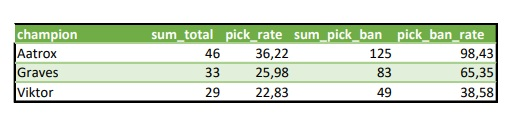
\includegraphics{3 amostras.jpg}
    \caption{Planilha Excel}
    \label{fig:enter-label}
\end{figure}

\begin{flushleft}
\textbf{Aatrox:}
\end{flushleft}

\begin{itemize}
  \item \textbf{sum\_total (46):} A pontuação total de Aatrox é relativamente alta, o que sugere uma presença significativa nas métricas consideradas em PC1.
  \item \textbf{pick\_rate (36.22\%):} A taxa de escolha de Aatrox é substancial, de modo que indica que ele é frequentemente escolhido durante as partidas, o que contribui positivamente para a variação em PC1.
  \item \textbf{sum\_pick\_ban (125):} A pontuação de escolha e banimento combinada é considerável, de forma a destacar a popularidade e relevância estratégica de Aatrox nas partidas.
  \item \textbf{pick\_ban\_rate (98.43\%):} A taxa combinada de escolha e banimento é elevada, o que indica que Aatrox é não apenas escolhido com frequência, mas também banido, de forma a consolidar sua importância estratégica.
\end{itemize}
\pagebreak


\begin{flushleft}
\textbf{Graves:}
\end{flushleft}

\begin{itemize}
  \item \textbf{sum\_total (33):} A pontuação total de Graves é menor em comparação com Aatrox, o que sugere uma presença moderada nas métricas relevantes para PC1.
  \item \textbf{pick\_rate (25.98\%):} Graves possui uma taxa de escolha considerável, e indica uma presença significativa nas partidas, mas menor do que Aatrox.
  \item \textbf{sum\_pick\_ban (83):} A pontuação combinada de escolha e banimento é moderada, o que sugere uma importância estratégica razoável, mas menor em comparação com Aatrox.
  \item \textbf{pick\_ban\_rate (65.35\%):} A taxa combinada de escolha e banimento é relativamente alta, de modo que indica que Graves é uma escolha e banimento estratégicos comuns.
\end{itemize}

\begin{flushleft}
\textbf{Viktor:}
\end{flushleft}

\begin{itemize}
  \item \textbf{sum\_total (29):} A pontuação total de Viktor é a mais baixa entre os três campeões, o que indica uma presença mais limitada nas métricas relevantes para PC1.
  \item \textbf{pick\_rate (22.83\%):} Viktor possui uma taxa de escolha inferior em comparação com Aatrox e Graves, de forma a sugerir uma presença menos frequente nas partidas.
  \item \textbf{sum\_pick\_ban (49):} A pontuação combinada de escolha e banimento é a mais baixa, o que torna uma importância estratégica relativamente menor em comparação com os outros campeões.
  \item \textbf{pick\_ban\_rate (38.58\%):} A taxa combinada de escolha e banimento é menor, de modo que se destaque que Viktor é escolhido e banido com menos frequência em comparação com Aatrox e Graves.
\end{itemize}

Ou seja, de acordo com a figura 4, tem-se Aatrox no topo do gráfico, Graves ao meio e Viktor no canto inferior esquerdo, portanto, o PC1 leva em conta o quanto um campeão é presente de forma a ser banido e também escolhido.


\begin{figure}[h]
Na figura 6 abaixo temos o grafico de coluna referente aos loadings de PC2:
    \centering
    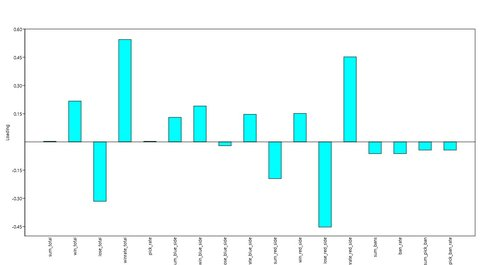
\includegraphics{LoadingsPC2 (1).jpg}
    \caption{Ferramenta PAST}
    \label{fig:enter-label}
\end{figure}
\pagebreak
Em relação a PC2, que representa a segunda maior fonte de variação, as duas variáveis com os maiores valores são:\\

1. \textbf{winrate\_total (0.54):} Indica a taxa de vitórias total, tal que sugere uma forte influência na variação ao longo do segundo componente principal.\\

2. \textbf{winrate\_red\_side (0.45):} Reflete a taxa de vitórias específica do lado vermelho (red side) do jogo, de forma a contribuir para a variação ao longo do segundo eixo principal.\\

Adicionalmente, é importante observar que as variáveis com pesos negativos também desempenham papéis significativos na análise:\\

3. \textbf{lose\_total (-0.32 em PC1):} Indica uma contribuição negativa significativa para a variação ao longo da direção principal, o que sugere que uma contagem elevada de derrotas totais reduz os valores de PC1.\\

4.  \textbf{lose\_red\_side (-0.45 em PC2):} Reflete uma influência negativa na variação ao longo do segundo componente principal, de modo que sugere que uma contagem alta de derrotas específicas do lado vermelho diminui os valores de PC2.\\

Essas observações destacam a importância não apenas das variáveis com pesos positivos, mas também das variáveis com pesos negativos na interpretação das principais direções de variação durante a análise PCA.
\pagebreak
\begin{figure}[h]
Agora ao analisar a relação de PC2 com PC2 em um gráfico gera-se a seguinte figura abaixo:
    \centering
    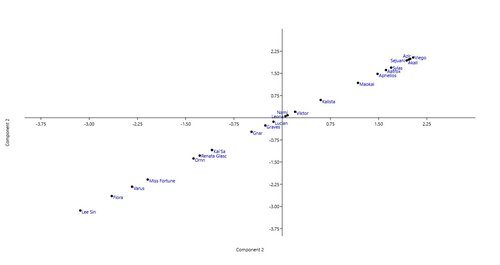
\includegraphics{pc2pc2 (1).jpg}
    \caption{Ferramenta PAST}
    \label{fig:enter-label}
\end{figure}
\begin{figure}[h]
Novamente para compreensão, serão selecionados 3 das amostras para analisar seus valores burtos como feito na figura abaixo, em vermelho estão as variáveis que escalam de forma negativa enquanto em amarelo as positivas:
    \centering
    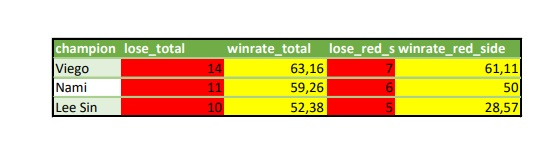
\includegraphics{3 amostras2.jpg}
    \caption{Planilha Excel}
    \label{fig:enter-label}
\end{figure}


Foram selecionados as 3 amostras mais extremas, Viego no topo do gráfico, Nami ao centro e Lee Sin na parte inferior esquerda, ao observar os valores e o plot temos que:\\

\begin{itemize}
    \item \textbf{Viego:}
    \begin{itemize}
        \item No componente 2 (PC2), Viego apresenta valores mais altos, de modo a indicar uma contribuição positiva significativa para a variação ao longo do segundo componente principal. Essa influência positiva é impulsionada pela sua alta taxa de vitórias total (winrate\_total = 63.16\%) e pela sólida taxa de vitórias específica do lado vermelho (winrate\_red\_side = 61.11\%).
    \end{itemize}
    \pagebreak
    
    \item \textbf{Nami:}
    \begin{itemize}
        \item Em PC2, Nami possui valores moderados, de forma a refletir uma contribuição positiva para a variação ao longo do segundo componente principal. Isso se deve à sua boa taxa de vitórias total (winrate\_total = 59.26\%) e à taxa de vitórias específica do lado vermelho (winrate\_red\_side = 50\%). Embora esses fatores contribuam para valores positivos em PC2, eles não são tão pronunciados quanto os de Viego.
    \end{itemize}
    
    \item \textbf{Lee Sin:}
    \begin{itemize}
        \item Lee Sin apresenta valores mais baixos em PC2, de modo que indique uma contribuição positiva menos intensa para a variação ao longo do segundo componente principal. Isso ocorre devido à sua taxa de vitórias total (winrate\_total = 52.38\%) e à taxa de vitórias específica do lado vermelho (winrate\_red\_side = 28.57\%). Embora contribuam de forma menos intensa, esses elementos ainda influenciam positivamente PC2.
    \end{itemize}
\end{itemize}

\textbf{} O componente 2 é influenciado positivamente por campeões com taxas de vitórias sólidas, especialmente quando jogados no lado vermelho. Viego destaca-se como o campeão com a maior contribuição positiva para a variação em PC2, seguido por Nami e Lee Sin com contribuições moderadas, que considera tanto vitórias quanto derrotas.

\section{Plotagem}

Com base nas análises, pode ser observado que o PC1 representa a presença de um campeão de forma a ser banido e escolhido, conforme visto na Figura 4, onde Aatrox ocupa o topo, Graves fica no meio e Viktor está no canto inferior esquerdo. Isso sugere que o PC1 está relacionado à popularidade e impacto estratégico de cada campeão nas partidas.\\

Por outro lado, o componente 2 (PC2) é influenciado positivamente por campeões com taxas de vitórias sólidas, especialmente quando jogados no lado vermelho. Viego se destaca como o campeão com a maior contribuição positiva para a variação em PC2, seguido por Nami e Lee Sin, ambos com contribuições moderadas. Essa análise leva em consideração tanto as vitórias quanto as derrotas dos campeões.\\

O PC1 reflete a presença e importância estratégica de um campeão no jogo, enquanto o PC2 destaca a performance em termos de vitórias e derrotas, especialmente quando jogados no lado vermelho. Essas conclusões proporcionam as características e impacto dos campeões nas partidas.
\pagebreak\\
\begin{figure}[h]
Ao analisar a figura abaixo que se tem pela relação de PC1 com PC2, pode ser observado a dispersão causada entre os dados.
    \centering
    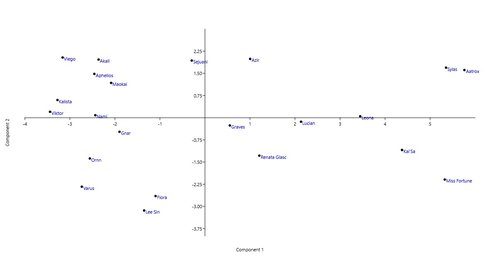
\includegraphics{plot (1).jpg}
    \caption{Scatter plot no PAST}
    \label{fig:enter-label}
\end{figure}\\
Se forem observados o Aatrox e Sylas, que se encontram no extremo direito do eixo X (PC1), podem ser interpretados como campeões frequentemente escolhidos e banidos, que indica uma presença significativa nas partidas, Além disso, eles também estão em posições consideráveis altas do eixo Y (PC2), de modo a indicar grandes valores nas taxas de vitórias.

Em outra perspectiva, Viego e Akali, estão no extremo esquerdo do eixo X (PC1) e no topo do eixo Y (PC2), significa que foram campões mais ausentes durante o campeonato, porém  podem ser interpretados como campeões com altas taxas de vitórias, destacando-se ainda mais quando no lado vermelho. Por outro lado, Lee Sin e Fiora, de modo a estarem abaixo no eixo Y (PC2) e à esquerda no eixo X (PC1), podem ser interpretados como campeões com taxas de vitórias menos expressivas e menos presença durante o campeonato.
\section{Conclusão}
A análise de componentes principais (PCA) emerge como uma ferramenta indispensável na moldagem de formações estratégicas no cenário competitivo de esportes. Nesse ambiente dinâmico, onde cada decisão pode alterar drasticamente o rumo de uma partida, a compreensão aprofundada dos dados é essencial. Ao se considerar o crescente mercado e a profissionalização do esporte, a aplicação do PCA destaca-se como um diferencial para equipes que buscam maximizar seu potencial.

Esta análise de campeões em esportes eletrônicos, como League of Legends, o PCA pode revelar padrões de desempenho que vão além das estatísticas convencionais. Por exemplo, identificar que campeões específicos, posicionados no extremo do eixo x (PC1), são altamente escolhidos e, ao mesmo tempo, situados no extremo do eixo y (PC2), apresentam índices de vitórias notáveis. Isso sugere uma relação direta entre popularidade e eficácia, informação crucial para estrategistas.

A expansão do mercado esportivo global traz consigo uma necessidade crescente de abordagens analíticas avançadas. A adaptabilidade do PCA permite sua aplicação em diversas áreas, desde a análise de desempenho de jogadores até a avaliação de estratégias de equipe. No contexto dos esportes eletrônicos, entender quais campeões impactam mais nos resultados pode orientar as decisões de escolha e banimento, de modo a influenciar diretamente o curso das partidas.

Assim, o PCA não apenas oferece uma visão aprofundada do desempenho atual, mas também permite prever tendências e ajustar estratégias para competições futuras. Em última análise, ao analisar de perto os campeões mais impactantes e suas relações complexas, as equipes podem aprimorar sua tomada de decisões e fortalecer sua posição no competitivo cenário esportivo.

\section*{Referências}
O estudo está disponivel no github no seguinte link: https://github.com/mirandalouco/PCA-Gustavo-Miranda.git\\\\
Para a escrita, e entendimento do assunto foram utilizados artigos produzidos por universidades federais como: https://www.cin.ufpe.br/~aluizioa/RN/RN-12-PCA.pdf\\\\
Para a normalização dos dados foram usadas como referenciais:\\\\
Normalização em Machine Learning: Ciência e Dados https://www.cienciaedados.com/normalizacao-em-machine-learning/ \\\\
Normalização de variáveis - UFSC https://geam.paginas.ufsc.br/files/2020/02/feature-scaling.pdf

\end{document}
